\documentclass{article}

\usepackage[utf8]{inputenc}

% Packages
\usepackage{amsmath,amssymb}
\usepackage{bm}% boldmath
\usepackage{listings} % Code block (source code) \begin{lstlisting} 
\usepackage{natbib}
\usepackage{graphicx}
\usepackage{lmodern}
\usepackage[usenames,dvipsnames,svgnames,table]{xcolor}
\usepackage[textwidth=16cm,textheight=23cm]{geometry}

%\usepackage{inconsolata} % New monospace font

% URL
\usepackage{url}
\usepackage[colorlinks=true, a4paper=true, pdfstartview=FitV, linkcolor=blue, citecolor=blue, urlcolor=blue]{hyperref}

% Figures
\usepackage[font=small, labelfont=bf]{caption}
\usepackage{subfig} % Subfigures. Uses \subfloat[captions text]{figure}

% Tables
\usepackage{booktabs}   % Allows the use of \toprule, \midrule and \bottomrule in tables for horizontal lines
\newcommand{\ra}[1]{\renewcommand{\arraystretch}{#1}} % spaces in tables

% Itemize
\usepackage{enumitem}

% Commands
%\newcommand{\code}[1]{\texttt{#1}} % \code{inline code}
\newcommand{\code}[1]{{\small\ttfamily #1}} % \code{inline code}
\newcommand{\expval}[1]{\langle #1 \rangle} %
\renewcommand{\theequation}{\arabic{section}.\arabic{equation}} % Book format equation
\renewcommand{\thefigure}{\arabic{section}.\arabic{figure}} % Book format figure
\renewcommand{\vec}[1]{{\bf #1}} % Lars likes this better than arrow

% Set page attribution
\setlength{\parindent}{0pt}


% PSTRICKS
\usepackage{pstricks,pst-node,pst-tree} % includes graph additions
\usepackage{pst-pdf} % Compiles the pictures
\usepackage{pst-node}
\usepackage{pst-plot}
\usepackage{pst-3dplot}
%\usepackage{pstricks-add,babel}




\lstset{
language=Python,                        % Code langugage
commentstyle=\color{gray},              % Comments font
basicstyle=\small\ttfamily,             % Code font, Examples: \footnotesize, \ttfamily
keywordstyle=\bfseries\color{blue},
stringstyle=\color{orange},
numbers=left,                           % Line nums position
numberstyle=\tiny,                      % Line-numbers fonts
stepnumber=1,                           % Step between two line-numbers
numbersep=5pt,                          % How far are line-numbers from code
frame=none,                             % A frame around the code
tabsize=4,                              % Default tab size
captionpos=b,                           % Caption-position = bottom
breaklines=true,                        % Automatic line breaking?
breakatwhitespace=false,                % Automatic breaks only at whitespace?
showspaces=false,                       % Dont make spaces visible
showstringspaces=false,                 % Dont make spaces visible in strings
showtabs=false,                         % Dont make tabls visible
belowskip=8pt,
morekeywords={range, xrange},
% backgroundcolor=\color{yellow}
% emph={[2]root,base}
% morekeywords={one,two,three,four,five,six,seven,eight,
}


%commentstyle=\color{gray},              % Comments font
%basicstyle=\small,                      % Code font, Examples: \footnotesize, \ttfamily



%basicstyle=\footnotesize\ttfamily,
%keywordstyle=\bfseries\color{green!40!black},
%commentstyle=\itshape\color{purple!40!black},
%identifierstyle=\color{blue},
%stringstyle=\color{orange},







% ***************************************************
% HEADER INFORMATION

\title{Exercise 3}
\author{Molecular Statistics, Week 3}
\date{}

% ***************************************************

\begin{document}


% ***************************************************
% BEGIN DOCUMENT
% ***************************************************

\maketitle


\section{Introduction and Theory}

%Hello \code{for n in range(2)} \code{print "again"} Scientist.

In this exercise you are going to implement the Lennard-Jones potential in our 2D simulation.
Figure \ref{fig:potentials} shows the three different potentials we've encountered so far.

\begin{figure}[h!]
\begin{center}
    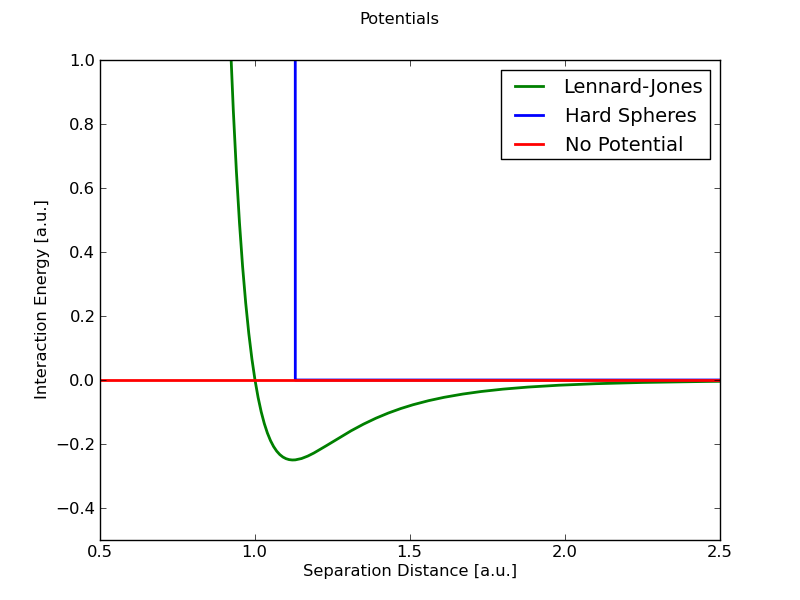
\includegraphics[width=0.75\textwidth]{images/potentials.png}
    \caption{The three different potentials we've encountered so far.}
    \label{fig:potentials}
\end{center}
\end{figure}


\subsection{The Lennard-Jones potential energy}

The Lennard-Jones potential energy between two interacting particles $i$ and $j$ is given by:
\begin{equation}
    U_{ij} = 4 \epsilon \left[ \left(\frac{\sigma}{r_{ij}} \right)^{12} - \left(\frac{\sigma}{r_{ij}} \right)^6 \right]
\end{equation}

Here $r_{ij}$ is the distance between the two particles.
For simplicity, we set $\epsilon = 1$ and $\sigma = 1$, in which case the energy is reduced to:
\begin{equation}
    U_{ij} = 4 \left[ \left(\frac{1}{r_{ij}} \right)^{12} - \left(\frac{1}{r_{ij}} \right)^6 \right]
\end{equation}

The total potential energy of the system is then;
\begin{equation}
    U_{\mathrm{Total}}
    = \sum_{i>j} U_{ij}
    = 4 \sum_{i>j} \left[ \left(\frac{1}{r_{ij}} \right)^{12} - \left(\frac{1}{r_{ij}} \right)^6 \right] \label{eq:total_energy}
\end{equation}

which computationally requires a double loop over each particle interaction.


% You should now be able to see how the summation $\sum_{i>j}$ requires a double loop over all particles in your code. These usually look
% something like:
% 
% \begin{lstlisting}[language=python]
% energy = 0.0
% for i in range(n_particles):
%     for j in range(n_particles):
%         if i > j:
%             energy = energy + ...
% \end{lstlisting}

\subsection{Inter-particle forces in the Lennard-Jones potential}

In the past two exercises, the total momentum of the particles was conserved.
However in the Lennard-Jones potential, we must calculate the force exerted by the particles upon each other, and use the forces to update the positions and velocities of the particles.
First, recall how we are able to calculate the force \textbf{F} using the energy gradient:

\begin{equation}
    \mathbf{F} = -\nabla U = -\left( \frac{\partial U}{\partial x_1},\ \frac{\partial U}{\partial y_1},\  \frac{\partial U}{\partial x_2},\ \frac{\partial U}{\partial y_2},\ \ldots\ ,\frac{\partial U}{\partial x_n},\ \frac{\partial U}{\partial y_n}\right)
    \label{eq:force}
\end{equation}

The $x$-components of the force between two interacting particles $i$ and $j$ are:

\begin{align}
    -\frac{\partial}{\partial x_i} U_{ij} &= -48\ \frac{x_j - x_i}{r^2_{ij}}\left[ \left(\frac{1}{r_{ij}} \right)^{12} - 0.5 \left(\frac{1}{r_{ij}} \right)^6 \right] \\
    -\frac{\partial}{\partial x_j} U_{ij} &=  48\ \frac{x_j - x_i}{r^2_{ij}}\left[ \left(\frac{1}{r_{ij}} \right)^{12} - 0.5 \left(\frac{1}{r_{ij}} \right)^6 \right]
\end{align}

The $y$-components are, of course, defined the same way.

\subsection{The Velo-Verlet solver}

The Velocity Verlet (Velo-Verlet) solver is one of many ways to go about integrating the motion of particles.
The Velo-Verlet algorithm updates the forces, velocities and positions at the same time.
The Velo-Verlet equations for integrating the positions ($r$) and velocities ($v$) are given the acceleration ($a$), for the $x$-direction of one particle:
\begin{eqnarray}
    r_x(t+dt)   &=& r_x(t) + dt \cdot v_x(t) + 0.5 \cdot dt^2 \cdot a_x(t) \label{eq:velo_pos} \\
   %x(t + dt)   &=& x(t) + dt\ v_x(t) + 0.5\ dt^2\ a_x(t) \label{eq:velo_pos} \\
    v_x(t + dt) &=& v_x(t) + 0.5 \cdot dt \cdot \left [ a_x(t) + a_x(t+dt) \right ] \label{eq:velo_vel}
\end{eqnarray}

In out simultation, we will set the mass of the particles to $1$, so the acceleration is equal to the force (Newtons 2nd law).
Let's recap: The Velo-Verlet algorithm uses the forces,
velocities and positions from the current time step to calculate the forces,
velocities and positions for the next time-step.
In short it is a three-step procedure:

\begin{enumerate}
    \item Calculate new positions, using Eq. \ref{eq:velo_pos}
    \item Calculate new forces, using Eq. \ref{eq:force}
    \item Calculate new velocities, using Eq. \ref{eq:velo_vel}
\end{enumerate}

The resulting forces, velocities and particle positions are then saved, and used as input for the next Velo-Verlet integration step.

\newpage
\clearpage
\section{Exercise}

Firstly, you will need to write the relevant code/functions to calculate the Lennard-Jones potential energy for a given system.

\begin{enumerate}

    \item Create a new file called \code{week3.py}.

    \item Define a function called \code{lennard\_jones()}, that takes positions and number of particles as parameters.

    \item Loop over all particle interaction (double loop over $i$ and $j$ particles) and calculate the total energy using eq. \ref{eq:total_energy}.

\end{enumerate}

When you think you have written the Lennard-Jones energy function properly,
it's time to test whether your function works correctly or not.
Define two lists:

\begin{lstlisting}[language=python]
n_particles = 2
pos_x_test = [0.0, 0.0]
pos_y_test = [0.0, 1.4]
\end{lstlisting}

\begin{enumerate}[resume]

    \item Now call the Lennard-Jones function with the two lists as arguments and print the result.
        If your energy function works, the resulting energy should be -0.4607.

\end{enumerate}

Next, we will extend the Lennard-Jones (LJ) function to also calculate the forces.
In our 2D system the force has $x$- and $y$-components for each particle.
So for this it would be natural to extend your code to store the $x$- and $y$-components in two lists called \code{force\_x} and \code{force\_y}, just like the velocities.

\begin{enumerate}[resume]

    \item In the LJ function, initialize two new lists for the forces, \code{force\_x} and \code{force\_x}, containing only zeros, with the length equal to the number of particles.
    {\em Hint:}

\begin{lstlisting}
force_x = [0.0 for i in range(n_particles)]
\end{lstlisting}

    \item In the loop when calculating the energy, insert code to calculate the force for each interaction and update the force lists with the corresponding interaction force, from eq. \ref{eq:force}.
        Use the following code as inspiration:

\begin{lstlisting}
for i in range(n_particles):
    for j in range(n_particles):
        if i > j:
            energy = energy + ...

            force_x[i] = force_x[i] + ...
            force_y[i] = force_y[i] + ...

            force_x[j] = force_x[j] + ...
            force_y[j] = force_y[j] + ...
\end{lstlisting}

    \item Use the position test lists from the previous question and calculate the forces and energies.
        The function should return \code{force\_x[0]} = 0.0 and \code{force\_y[0]} = 1.6720.

\end{enumerate}

Next is to implement the Velo-Verlet solver.
The Velo-Verlet solver needs the current forces, velocities and particle positions as input.
Your code already initializes the velocities and positions, but doesn't calculate the initial forces.\\

Last week we used random $x$- and $y$-coordinates, within a (-1, 1) box.
However, when we are working with a potential it is not a good idea to use completely random coordinates, as the initial gradient might be unphysically large.
And because we are working with a potential with $\sigma = 1$, we will need to expand the box by setting \code{box\_width = 10.0} instead of 1 since if two particles end up starting with $r_{ij} < 1$ (see figure \ref{fig:potential_energy}), the system would 'explode'.\\

Because of this we want to re-write the \code{initialize\_particles}-function from last week to initialize the particles in a nice grid, instead of random positions.
We have completed the following code for your convenience.

\begin{lstlisting}
def initialize_particles(n_particles, box_width):
    """ Initialize particles in a grid
    """
    
    # Get the smallest grid that all particles will fit in.
    sqrt_npart = int(np.ceil(np.sqrt(n_particles)))

    X = []
    Y = []

    # Arrange sqrt_npart**2 particles in a grid
    for j in range(sqrt_npart):
        X += [i for i in range(sqrt_npart)]
        Y += [j for i in range(sqrt_npart)]

    # Remove excess particles created
    X = X[:n_particles]
    Y = Y[:n_particles]

    # Rescale particle positions to fit in the box.
    for i in range(n_particles):
        X[i[ = (X[i] - 0.5 * sqrt_npart) * 1.0/sqrt_npart * box_width * 1.8
        Y[i] = (Y[i]) * 1.0/sqrt_npart * box_width * 0.8

    # Initialize particle velocities
    Vx = [2 * (random.random() - 0.5) for i in range(n_particles)]
    Vy = [2 * (random.random() - 0.5) for i in range(n_particles)]

    # Inititalize particle forces
    Fx, Fy, energy = lennard_jones(X, Y)

    return X, Y, Vx, Vy, Fx, Fy

\end{lstlisting}

\begin{enumerate}[resume]
    \item Include the above \code{initialize\_particles} function in your code, set \code{box\_width} to 10.0 and initialize the positions, velocities and forces.
    {\em Note:} You don't need to understand everything in detail in the initializing code.
\end{enumerate}

Now it's time to implement the Velo-Verlet solver.

\begin{enumerate}[resume]

    \item Create a new function and name it \code{velo\_verlet}.
        Have the function take positions, velocities, forces, number of particles and dt as arguments.

    \item The new function should return the positions, velocities, forces and the energy of the system.

    \item Implement the three steps of the Velo-Verlet integration algorithm.
        Which means, implement the following code in your \code{velo\_verlet}-function.

\begin{lstlisting}
# Step 1: Update the positions
for i in range(n_particles):
    pos_x[i] = pos_x[i] + dt * vel_x[i] + 0.5 * dt * dt * force_x[i]

# Remmeber the previous forces
force_x_old = copy.copy(force_x)

# Step 2: Calculate the new forces and energy
force_x, force_y, energy = lennard_jones(pos_x, pos_y)

# Step 3: Calculate the new velocities.
for i in range(n_particles):
    vel_x[i] = vel_x[i] + 0.5 * dt * (force_x_old[i] + force_x[i])

\end{lstlisting}

    \item Correct the particles if they collide with the wall (just like week 1 and 2).

    \item After the initialization of the particles, insert the loop over \code{range(n\_steps)}, this time with the \code{velo\_verlet} function, instead of \code{simulate\_step}.
        This should look something like;

\begin{lstlisting}
for n in range(n_steps):
    X, Y, Vx, Vy, Fx, Fy, energy = velo_verlet(X, Y, Vx, Vy, Fx, Fy, dt)
\end{lstlisting}

    \item Your code should now run a simulation of a Lennard-Jones 2D gas.
        Save a video of the particle movements using the following constants, and convince yourself that your code is working properly
        {\em Note:} Use \code{video.save('simulation',box\_width)} to save a video with a box width differing from 1.

\begin{lstlisting}
box_width = 10.0
n_particles = 42
n_steps = 5000
dt = 0.001
\end{lstlisting}

\end{enumerate}



Let's try and see how your simulation works.

\begin{enumerate}[resume]

    \item store the energy during the simulation, in a file. Write the energy every 5th step.
        
    \item Plot the energy using another file and see if the potential energy is roughly conserved over time.
        If your time-step is too large or too small, this might not be the case.
        A healthy simulation looks something like Figure \ref{fig:potential_energy}

    \item Try and run the simulation with a small and a large $dt$ value. 
        Can you make the simulation break down this way?
        And how does $dt$ influence the number of steps it takes to equilibrate the potential energy?

\end{enumerate}

\begin{figure}[htb]
  \centering
  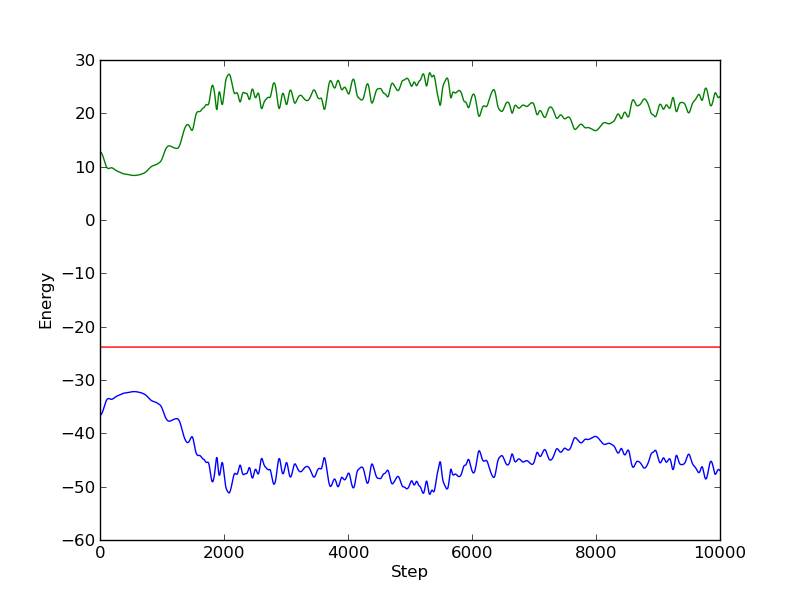
\includegraphics[width=0.75\textwidth]{images/potential_energy.png}
  \caption{Potential energy during a "healthy" MD simulation in a Lennard-Jones potential.}
  \label{fig:potential_energy}
\end{figure}


% If you finish early, do these exercises before you leave:\\
% 
% Multiply the random velocities in the initialize\_particles function by a small scaling factor (i.e. a small number $< 1$).
% This lowers the average velocities of the particles and corresponds to running the simulation at a lower temperature.
% Recall the Maxwell-Boltzmann distribution of the mean speed of particles in a gas:
% 
% \begin{align}
%     \langle v \rangle = \sqrt{ \frac{8\ R \ T}{\pi\ M}}
% \end{align}
% 
% Here $R$ is the gas constant, $T$ the temperature and $M$ the molar mass of the gas.\\
% 
% Answer the following two questions:
% 
% \begin{enumerate}
%     \item Can you find a scaling factor so the particles behave more like a liquid rather than a gas? 
%     \item What property of the Lennard-Jones is very important if you want to simulate aggregation of particles?
% \end{enumerate}


% ***************************************************
% END DOCUMENT
% ***************************************************

\end{document}

